



\subsection{Messversuch - Ablauf EMG}

\subsubsection{Elektroden anbringen}

Der Versuchsablauf begann mit der Vorbereitung des Probanden, bei der eine EMG-Elektrode an einem zuvor definierten Muskel des Quadrizeps angebracht wurde. Die Messung wurde schrittweise für drei verschiedene Muskeln des Quadrizeps durchgeführt: den Vastus medialis (innen), den Rectus femoris (mittig) und den Vastus lateralis (außen).

\begin{figure}
    \centering
    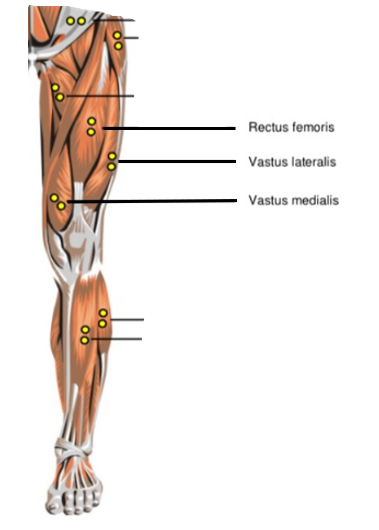
\includegraphics[width=0.5\linewidth]{img/EMG Muskeln.png}
    \caption{EMG Messung Elektroden}
    \label{EMG-Messung-Elektroden}
\end{figure}

Zu Beginn der Messreihe wurde die Elektrode beispielsweise an beiden Beinen am Vastus medialis platziert, bevor sie nach Abschluss der ersten Messung an den nächsten Muskel versetzt wurde. Dieses Vorgehen wurde nacheinander für beide Beine wiederholt.\\
\\
\subsubsection{Kalibrierung}
Nachdem die Elektrode positioniert war, stellte sich der Proband auf die zuvor angefertigte Fußschablone, um eine reproduzierbare Standposition einzunehmen. Das Messsystem Noraxon wurde verwendet, um die Versuchsperson auszuwählen und die genaue Platzierung der Elektrode am jeweiligen Muskel zu dokumentieren. Anschließend erfolgte die Kalibrierung der Muskelspannungskurve, bei der die Ausgangswerte auf null gesetzt wurden, um Störsignale zu eliminieren und eine präzise Messung der Muskelaktivität zu gewährleisten.\\
\\
\subsubsection{Kniebeugen}
Nach der erfolgreichen Kalibrierung begann der Proband mit der Durchführung von sechs Kniebeugen. Zwischen jeder Kniebeuge pausierte er kurz in der Streckung, bevor er die nächste Bewegung startete.
\subsubsection{Datenverarbeitung}
Nachdem die Messung gestoppt wurde, sind die aufgezeichneten EMG-Signale vor der Marker-Setzung im Noraxon-System geglättet worden. Diese Glättung sorgte dafür, dass kleine Störungen oder Artefakte in der Rohdatenaufzeichnung entfernt wurden, wodurch die Signalqualität für die spätere Auswertung verbessert wurde.\\
Nach der Signalglättung wurden im System Marker gesetzt, die zwei wesentliche Phasen definierten: die Ruhephase im Stand und die Aufwärtsbewegung, in der die höchste Muskelspannung erreicht wurde. Diese Marker ermöglichten eine zielgerichtete und strukturierte Auswertung der relevanten Bewegungsabschnitte.
Parallel dazu zeichnete eine synchronisierte Kamera die Bewegungen des Probanden auf. Die Kamera nahm bei jedem gesetzten Marker ein Bild auf, wodurch die visuellen Informationen der Bewegung mit den EMG-Daten verknüpft wurden. Dieses Zusammenspiel von Videoaufnahmen und EMG-Messungen erleichterte die anschließende Analyse der Muskelaktivität.
\subsubsection{Wiederholung für die anderen Muskeln}
Nach Abschluss der ersten Messung wurden die Elektroden an den nächsten Muskel versetzt. Der gesamte Prozess – von der Platzierung der Elektroden über die Kalibrierung und Durchführung der sechs Kniebeugen bis hin zur Signalglättung – wurde für jeden der drei Zielmuskeln des Quadrizeps wiederholt. Dies gewährleistete eine vollständige und differenzierte Erfassung der Muskelaktivität.
Sobald alle Messungen abgeschlossen waren, führte das Noraxon-System eine umfassende Analyse der gesammelten Daten durch. Diese umfasste die Darstellung der geglätteten Muskelspannungsprofile, die Auswertung der Marker-basierten Phasen sowie den Vergleich der Aktivitätsmuster zwischen den unterschiedlichen Muskeln. Die Ergebnisse bildeten die Grundlage für weiterführende Analysen und die Interpretation der Muskelaktivität während der Kniebeugen sicherzustellen.

